\section{Python}
This section will shortly give an overview of the Python programming language version 3.5.1.
This section is based on \citet{python_docs}.

The Python programming language was created by Guido van Rossum in the early 1990s and is to this day the main author.
As the language has grown there are obviously many more contributors and everyone can contribute as Python is Open Source.

\subsection{Control Structures}
The python programming language has three control structures, \texttt{if}, \texttt{while} and \texttt{for}.
In the following they are presented as simple examples and a figure showing the possible flow.

\paragraph{\texttt{If}}
The \texttt{if} control structure has several statements:
\begin{enumerate}
\item A simple \texttt{if} statement
\item An \texttt{if-else} statement
\item An \texttt{if-elif-else} statement
\end{enumerate}
The \texttt{if} and \texttt{elif} statements contain a condition which is evaluated to either true or false.
If the condition is true the body of the statement is evaluated if it is false the interpreter will jump to the code after the body.

\begin{figure}
  \centering
  \begin{subfigure}[b]{0.4\textwidth}
    \begin{lstlisting}[style=python, caption={Code example.}, label={python:if:simple:code}]
if True:
    x = 0
    \end{lstlisting}
  \end{subfigure}
  ~ %add desired spacing between images, e. g. ~, \quad, \qquad, \hfill etc. 
  %(or a blank line to force the subfigure onto a new line)
  \begin{subfigure}[b]{0.4\textwidth}
    \centering
    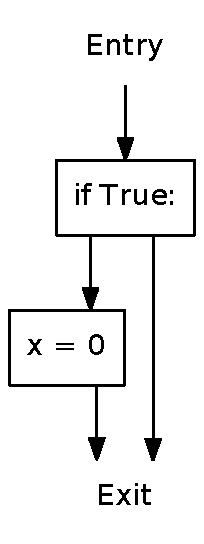
\includegraphics[scale=.5]{./figures/if.pdf}
    \caption{Possible flows.}
    \label{python:if:simple:flow}
  \end{subfigure}
  \caption{A simple \texttt{if} control structure containing one \texttt{if} statement.}
  \label{python:if:simple}
\end{figure}

Taking a look at \cref{python:if:simple} we can see a simple \texttt{if} structure containing only one \texttt{if} statement.
The code, \cref{python:if:simple:code}, is an \texttt{if} statement with a condition, \texttt{True}.
If the condition holds the body is evaluated and if not the program moves on to the next piece of code.
This flow can be seen on \cref{python:if:simple:flow}.
